\documentclass[a4paper,12pt]{report}

\usepackage[cm-default]{fontspec}
\usepackage[russian]{babel}
\usepackage{amsmath,amssymb,amsthm}
\usepackage{multicol}
\usepackage{color}
\usepackage[top=20mm, bottom=20mm, left=25mm, right=15mm]{geometry}
\usepackage[colorlinks,filecolor=blue,citecolor=darkgreen,anchorcolor=pink]{hyperref}
\usepackage{tikz}
\usepackage{hologo}
\usepackage{graphicx}

\definecolor{darkgreen}{rgb}{0, 0.5, 0}
\definecolor{graylight}{rgb}{0.6, 0.6, 0.6}
\definecolor{mypink}{cmyk}{0, 0.7808, 0.4429, 0.1412}

\setmainfont{Times New Roman} 
\setsansfont{CMU Sans Serif}
\setmonofont{CMU Typewriter Text}

\newcommand{\mono}[1]{{\small\texttt{#1}}}

\newtheorem{Лемма}{Лемма}
\newtheorem{Определение}{Определение}
\newtheorem{Теорема}{Теорема}

\author{Булгаков Виталий}
\title{Алгоритм полиномиального времени для взлома базовой криптосистемы Меркла-Хеллмана}

\begin{document}
\thispagestyle{empty}

\begin{center}

\sc
ФЕДЕРАЛЬНОЕ  ГОСУДАРСТВЕННОЕ АВТОНОМНОЕ
ОБРАЗОВАТЕЛЬНОЕ УЧРЕЖДЕНИЕ ВЫСШЕГО ОБРАЗОВАНИЯ
«НАЦИОНАЛЬНЫЙ ИССЛЕДОВАТЕЛЬСКИЙ УНИВЕРСИТЕТ
«ВЫСШАЯ ШКОЛА ЭКОНОМИКИ»
\end{center}

\begin{center}
\bf Московский институт электроники и математики им.~А.Н.~Тихонова
\end{center}

\vspace{1cm}

\begin{center}
Булгаков Виталий Валерьевич
\end{center}

\vspace{1cm}

\begin{center}
\bf Перевод статьти Ади Шамира "Алгоритм полиномиального времени для взлома базовой криптосистемы Меркла-Хеллмана"
\end{center}

\vspace{10mm}

\begin{center}
Курсовая работа \par
по специальности 10.05.01 «Компьютерная безопасность» \par
студента образовательной программы специалитета
\end{center}

\vfill

\begin{multicols}{2}
\begin{flushleft}
~Студент\par\:\par
\begin{tabular}{c}
\underline{\hspace{8em}} \vspace{-2mm}\\
{\tiny {\color{graylight}подпись}}
\end{tabular}
\begin{tabular}{c}
\underline{\hspace{2em}Булгаков В.В.\hspace{1em}}\\
{\tiny{\color{graylight} ФИО}}
\end{tabular}
\end{flushleft}

\begin{flushright}
Преподаватель

доцент
\end{flushright}

\begin{tabular}{c}
\underline{\hspace{8em}} \vspace{-1mm}\\
{\tiny {\color{graylight}подпись}}
\end{tabular}
\begin{tabular}{c}
\underline{\hspace{2em}Нестеренко А.Ю.\hspace{1em}} \vspace{-1mm}\\
{\tiny{\color{graylight} ФИО}}
\end{tabular}
\end{multicols}

\vfill
\begin{center}Москва, 2021 г.\end{center}

\newpage

\tableofcontents

\chapter{Аннотация}

\textbf{Криптосистема Меркла-Хеллмана является одной из двух основных криптосистем с открытым ключом, предложенных до сих пор. Здесь показано, что базовый вариант криптосистемы, в котором элементами открытого ключа являются кратными по модулю быстровозрастающие последовательности, может быть взломан за полиномиальное время.}

\chapter{Введение}

В 1976 году Диффи и Хеллман опубликовали свою новаторскую работу по криптографии с открытым ключом~\cite{hellman}. В их статье высказывалось предположение, что такие криптосистемы существуют, и рассматривались их потенциальные области применения, но не описывались фактические реализации. В конце 1976 и начале 1977 года были обнаружены две первые криптосистемы с открытым ключом (см.~\cite{mh,ral}). С тех пор было предложено множество вариантов и несколько новых криптосистем с открытым ключом, но по ряду причин эти первые две системы продолжают доминировать в этой области. Они были тщательно проанализированы, и
для их взлома был предложен ряд криптоаналитических атак. Однако все эти атаки вряд ли увенчаются успехом, если криптосистемы не будут значительно упрощены или размеры их ключей не будут уменьшены.

Мы описываем первую известную нам криптоаналитическую атаку, которая может взломать полноразмерный вариант одной из этих криптосистем в разумных временных и пространственных сложностях. Этот вариант известен как криптосистема Меркла-Хеллмана с одной итерацией, и он является самым простым (и, по-видимому, наименее безопасным) в семействе криптосистем с открытым ключом, предложенных в оригинальной статье Меркла и Хеллмана. Криптоаналитическая атака не применима напрямую к многоитерационной криптосистеме Меркла-Хеллмана, и поэтому криптографическая безопасность этих вариантов остается открытой проблемой.

Алгоритм прост в реализации и эффективен даже на микрокомпьютере. Он всегда останавливается после полиномиально большого количества шагов, но иногда может не сломать определенный ключ. Эвристические аргументы указывают на то, что такие сбои чрезвычайно редки, и они подтверждаются сотнями тестов, проведенных на полноразмерных ключах без единого сбоя.

Ряд контрмер может защитить криптосистему на основе рюкзака от конкретной атаки, рассмотренной здесь. Для некоторых из этих контрмер существуют контрмеры, которые могут активизировать атаку. Криптография - это бесконечная борьба между создателями кода и взломщиками кода, и эта статья не претендует на то, чтобы дать какие-либо окончательные ответы в этом смысле.

В главе \ref{ch::basic} представлен обзор криптосистемы Меркла-Хеллмана. В главе \ref{ch::informal} мы неформально описываем криптоаналитическую
атаку, а в главе \ref{ch::points} анализируем ее производительность. Обсуждение результатов приведено в главе \ref{ch::discussion}.

\chapter{Базовая криптосистема Меркла-Хеллмана}\label{ch::basic}

Открытый ключ шифрования в любой криптосистеме Меркла-Хеллмана представляет собой последовательность из $n$ натуральных чисел $a_1,\ldots,a_n$ (Типичное значение $n$ равно 100, а типичный размер каждого $a_i$ составляет 200 бит.) Для шифрования $n$-бит открытого текста, $X = x_1,\ldots,x_n,(x \in (0, 1)$, отправитель вычисляет зависящую от сообщения частичную сумму элементов $a_i$:
\[
\ b = \sum_{i = 1}^n x_i a_i,
\]

\noindent и отправляет зашифрованный текст $b$ получателю через (небезопасный) канал связи. И получатель, и потенциальный подслушивающий знают $a_1,\ldots,a_n$ и $b$, и они должны найти, какое подмножество элементов $a$, суммируется с $b$. Это пример проблемы с рюкзаком, которая, как известно, является недетерминированным полиномиальным временем (NP-полным). Чтобы сделать эту проблему, по-видимому, сложной (для подслушивающего), но на самом деле легкой (для получателя), последовательность $a_1,\ldots,a_n$ выбирается особым образом. Сначала получатель выбирает последовательность чисел $a_1',\ldots,a_n'$ для которых легко решить связанные экземпляры рюкзака. Затем он шифрует числа таким образом, что только он знает, как вернуть их в исходную форму. Наконец, он публикует зашифрованные числа $a_1,\ldots,a_n$ в качестве своего открытого ключа шифрования.

Есть много способов, с помощью которых можно выбрать простую последовательность действий, а затем замаскировать ее. Основная схема, предложенная в статье Меркла и Хеллмана основана на быстровозрастающих последовательностях и умножениях по модулю. Последовательность чисел $a_1',\ldots,a_n'$ \mono{увеличивается}, если каждое число в ней больше, чем сумма его предшественников:
\[
\ a > \sum_{j = 1}^{i - 1} a_j'.
\]

\noindent Для любой быстровозрастающей последовательности существует жадный алгоритм линейного времени для решения всех связанных с ним экземпляров рюкзака. Чтобы скрыть очевидную структуру такой последовательности, получатель случайным образом выбирает два числа, $M_0$ (модуль) и $U_0$ (множитель), такие, что $M_0$ больше суммы всех $a_i'$ и $U_i$ является относительно простым по отношению к $M_0$. Каждый $a_i'$ затем преобразуется в новое, случайно число между 0 и $M_0 - 1$ путем модульного умножения
\[
\ a_i \equiv U_0 \cdot a_i' (mod M_0),
\]

\noindent и новая последовательность, $a_1,\ldots,a_n$ публикуется в качестве ключа шифрования.

Чтобы показать, что асимптотическая сложность нашей криптоаналитической атаки полиномиальна, мы должны рассмотреть семейство криптосистем, размеры которых растут до бесконечности. Есть два основных параметра, которые мы должны учитывать: количество элементов в опубликованном ключе и их размеры. Если любой из них остается постоянным, существует тривиальный алгоритм полиномиального времени для решения связанных экземпляров рюкзака. Таким образом, мы делаем предположение, что размер модуля $M_0$ (и, следовательно, также размер элементов $a_i$) растет линейно с $n$. Если $d$ - константа пропорциональности $(1 < d < \infty)$, мы выбираем, чтобы $a_1'$ имел $dn - n$ битовое число,$a_i'$ должно быть $dn - n + i - 1$ бытным, и $M_0$ должно быть $dn$ битным (при необходимости $dn$ округляется до ближайшего целого числа). Меркл и Хеллман используют эту схему с $d = 2$ и $n = 100$, так что $a_i'$ увеличивается в размере от 100 до 199 бит, а $|M_0|$ равно 200. Параметр $d$ измеряет избыточность, введенную криптосистемой (т. е. соотношение между размерами зашифрованного текста и открытого текста). Сложность нашего алгоритма - это быстровозрастающая функция $d$, но для каждого фиксированного $d$ она полиномиальна от $n$.

\chapter{Неформальное описание алгоритма}\label{ch::informal}

Алгоритм, предложенный в этой статье, анализирует заданные числа $a_1',\ldots,a_n'$ и пытается найти пару лазеек(\mono{ориг. trapdoor pair}) натуральные числа $M$ и $W$ такие, что $W \cdot a_i (mod M)$ является быстровозрастающей последовательностью, и ее сумма меньше, чем $M$. Если известна какая-либо пара чисел с этими свойствами, то можно решить все экземпляры рюкзака, связанные с $a_1',\ldots,a_n'$ за линейное время. Поскольку $a_i$, были получены из быстровозрастающей последовательности путем модульного умножения, мы знаем, что существует по крайней мере одна такая пара (с $W_0 \equiv U_0^{-1}$(mod $M_0$)). Наш алгоритм находит некоторую пару лазеек, но не гарантируется, что он найдет исходный модуль и множитель, используемые при построении открытого ключа.

Алгоритм разделен на две части. В первой части алгоритм целочисленного программирования Ленстры~\cite{knuth} используется для нахождения нескольких небольших интервалов в [0, 1], таких что \mono{необходимым} условием для того, чтобы $M$ и $W$ были парой лазеек, является то, что отношение $W/M$ находится в таком интервале. Во второй части алгоритма мы используем тот факт, что приблизительно известно, что $W/M$ выполняет более точный анализ и делит каждый интервал на более мелкие подинтервалы, так что \mono{достаточным} условием для того, чтобы $M$ и $W$ были парой лазеек, является то, что их соотношение находится в таком подинтервале. По крайней мере, один из подинтервалов должен быть непустым, и, используя быстрый алгоритм диофантовой аппроксимации (алгоритм диофантового приближения)~\cite{cassels}, мы можем найти наименьшие $M$ и $W$, соотношение которых удовлетворяет этому условию.

\begin{figure}[h]
\centering
\begin{tikzpicture}[line width = 1pt, scale = 1]
\draw[-stealth] (0, 0) -- (0, 4.9) node[below right = 2pt] {$Wa_i\quad\left({\rm mod}\, M_0\right)$};
\draw[-stealth] (0, 0) -- (6.3, 0) node[above right] {$W$};
\foreach \i in {0, 1, 2, 3, 4}{\filldraw [black] (\i * 1.4, 0) circle (2pt);}
\foreach \i in {1, 2, 3, 4}{\draw[dashed] (\i *1.4, 0) -- (\i * 1.4, 3.8);}
\foreach \i in {0, 1, 2, 3}{\draw (0 + \i * 1.4,0) -- (1.4 + \i * 1.4, 3.8);}
\draw[dashed] (0, 3.8) -- (5.6, 3.8);
\filldraw [black] (0, 3.8)node[left] {$M_0$} circle (2pt);
\draw (5.6, 0) node[below] {$M_0$};
\end{tikzpicture}
\caption{}\label{fig 1}
\end{figure}


Пусть $M_0$ - (неизвестный) модуль разрядности $dn$, используемый при построении ключа шифрования. Теперь мы обобщаем определение пары лазеек, рассматривая произвольные реальные положительные значения $W$. График функции $Wa_i(mod M_0)$ для действительных множителей $0 \leq W \leq M_0$ имеет пилообразную форму, как показано на Рис. \ref{fig 1}. Наклон функции (за исключением точек разрыва) равен $a_i$, количество минимумов равно $a_i$, а расстояние между последовательными минимумами равно $M_0/a_i$ (что немного больше 1).

Рассмотрим теперь пилообразную кривую, связанную с $a_1$. Множитель $W_0$, обладает таким свойством, что $a_1' \equiv W_0 \cdot a_1 (mod M_0)$ составляет не более $2^{dn - n}$. Поскольку наклон кривой равен $a_1$, расстояние по горизонтали между $W_0$ и ближайшим минимумом кривой $a_1$ слева от нее не может превышать $2^{dn - n}/a_1 \approx 2^{-n}$. Неизвестный $W_0$, таким образом, должен быть чрезвычайно близок к некоторому минимуму пилообразной кривой $a_1$. К сожалению, даже если мы наложим ограничение на интегральность на $W$ (чего мы не делаем), для $W_0$ существует слишком много возможных значений, и мы не можем проверять их одно за другим.

Аналогичный анализ показывает, что $W_0$, также должен находиться на расстоянии \\ $2^{dn - n + 1}/a_2 \approx 2^{-n + l}$ от ближайшего минимума кривой $a_2$ слева от нее. Следовательно, два минимума кривых $a_1$ и $a_2$ должны быть очень близки друг к другу (минимум $a_2$ может быть до $2^{-n + l}$ слева или до $2^{-n}$ справа от минимума $a_1$ в зависимости от точного местоположения $W_0$). Это условие близости значительно уменьшает количество мест, в которых может находиться $W_0$, но в большинстве случаев оно все еще не характеризует его однозначно.

Аналогично, мы можем наложить больше пилообразных кривых на одну и ту же диаграмму. Тот факт, что $W_0$ близок к минимуму на каждой кривой, подразумевает, что все эти минимумы близки друг к другу, и поэтому вместо того, чтобы находить $W_0$, мы должны найти точки накопления минимумов различных кривых.

Существует простое эмпирическое правило, которое может помочь нам оценить, сколько пилообразных кривых должно быть проанализировано одновременно, прежде чем их набор точек накопления будет уменьшен до приемлемого размера. Обширные эксперименты показали, что эта оценка реалистична, но не надежна. Формальный анализ этого вопроса можно найти в главе \ref{ch::points}.

Пусть $l$ будет числом пилообразных кривых, которые мы накладываем на нашу диаграмму. Рассмотрим $p$-й минимум кривой $a_1$, которая расположена в точке $W = pM_0/a_1$. Ближайший минимум кривой $a_i$, может находиться в любом месте интервала
\[
\ [(pM_0 / a_1 - M_0 / 2a_i, pM_0 / a_1 + M_0 / 2a_i)],
\]

\noindent длина которого $M_0/a_i \approx 1$. Сделав разумное (но неочевидное) предположение о том, что фактические местоположения различных минимумов $a_i$, в этих интервалах являются независимыми случайными величинами с равномерным распределением вероятностей, мы можем оценить вероятность того, что минимумы кривых $a_2,\cdot,a_l$, все достаточно близки к $p$-му минимуму кривой $a_1$, на
\[
\ 2^{- n + 1} \cdot 2^{- n + 2}\ldots2^{- n + l - 1} \approx 2^{-ln+n+l^{2} / 2}.
\]

\noindent Поскольку мы должны учитывать $a_1$ возможных значений $p$, ожидаемое количество точек накопления равно
\[
\ 2_i \cdot 2^{-ln + n + l^{2} / 2} \approx 2^{dn - ln + n + l^{2} / 2}.
\]

\noindent и это значение меньше 1 всякий раз, когда
\[
\ (l - d - 1)n > l^{2} / 2.
\]

\noindent Когда $n$ достаточно велико, этому условию удовлетворяет 
\[
\ l > d + 1,
\]

\noindent и, таким образом, число $l$ является константой, которая зависит от $d$, но не от $n$. Утверждение о том, что ожидаемое количество точек накопления меньше 1, не следует понимать буквально, поскольку мы знаем, что одна точка накопления всегда существует по конструкции. Однако разумно предположить, что на практике “встроенная” точка не будет сопровождаться слишком большим количеством “случайных” точек, когда $l$ больше $d + 1$. В частности, когда $n = 100$ и $|M| = 200$, $l = 4$, кажется, является разумным кандидатом на количество пилообразных кривых, которые мы должны проанализировать.

Остаются две проблемы: как избавиться от $M_0$ (значение которого на самом деле неизвестно) и как найти точки накопления минимумов $l$ пилообразных кривых.

Ключевое наблюдение состоит в том, что расположение точек накопления на Рис. \ref{fig 1} зависит от \mono{наклонов} кривых, но не от их \mono{размеров}. Если мы разделим обе координаты на $i$-й кривой на $M_0$, мы получим пилообразную кривую функции $Va_i$ (mod 1), $0 \leq V < 1$, которая не зависит от $M_0$ как показано на Рис. \ref{fig 2}. В новой системе координат наклон кривой остается $a_i$, а количество минимумов остается $a_i$, но расстояние между последовательными минимумами уменьшается до $1 / a_i$. Исходный параметр $W_0$, заменяется новым параметром $V_0 = W_0 / M_0$ и допустимое расстояние между этим параметром и ближайшим минимумом кривой $a_i$ уменьшается примерно в $2^{dn}$ (от $2^{-n + i - 1}$ до $2^{-dn - n + i - 1}$).

Задача определения местоположения точек накопления $l$ минимума в новой системе координат может быть описана линейными неравенствами с $l$ интегральными неизвестными. Условия, при которых $p$-й минимум $a_1$, $q$-й минимум $a_2$, $r$-ый минимум $a_3$, и т.д. достаточно близкими друг к другу, являются

\begin{figure}[h]
\centering
\begin{tikzpicture}[line width = 1pt, scale = 1]
\draw[-stealth] (0, 0) -- (0, 4.9) node[below right = 2pt] {$Va_i\quad\left({\rm mod}\, l\right)$};
\draw[-stealth] (0, 0) -- (6.3, 0) node[above right] {$V$};
\foreach \i in {0, 1, 2, 3, 4}{\filldraw [black] (\i * 1.4, 0) circle (2pt);}
\foreach \i in {1, 2, 3, 4}{\draw[dashed] (\i *1.4, 0) -- (\i * 1.4, 3.8);}
\foreach \i in {0, 1, 2, 3}{\draw (0 + \i * 1.4,0) -- (1.4 + \i * 1.4, 3.8);}
\draw[dashed] (0, 3.8) -- (5.6, 3.8);
\filldraw [black] (0, 3.8)node[left] {$l$} circle (2pt);
\draw (5.6, 0) node[below] {$l$};
\end{tikzpicture}
\caption{}\label{fig 2}
\end{figure}

\begin{align*}
&p,q,r,\ldots,integers, & &1\leq p \leq a_1 - 1, \\
&-\epsilon_2 \leq p/a_1 - q/a_2 \leq \epsilon_2', & &1 \leq p \leq a_2 - 1, \\
&-\epsilon_3 \leq p/a_1 - r/a_3 \leq \epsilon_3', &  &1\leq r \leq a_3 - 1, \\
&\vdots &\vdots
\end{align*}

\noindent где $\epsilon_i$ и $\epsilon_i'$ представляют допустимые отклонения вправо и влево от $p/a_1$ соответственно. Умножая каждое двойное неравенство на его знаменатели, мы получаем эквивалентную систему

\begin{align*}
&p,q,r,\ldots,integers, & &1\leq p \leq a_1 - 1, \\
&-\delta_2 \leq pa_2 - qa_1 \leq \delta2', & &1 \leq q \leq a_2 - 1, \\
&-\delta_3 \leq pa_3 - ra_1 \leq \delta_3', &  &1\leq r \leq a_3 - 1, \\
&\vdots &\vdots
\end{align*}

\noindent что показывает, что значения $a_2, a_3, \ldots$ одновременно уменьшаются до малых абсолютных значений при умножении на $p$ и уменьшении mod $a_1$.

На Рис. \ref{fig 3} показан типичный увеличенный участок наложенной диаграммы в окрестности $W_0 / M_0$. Задача одновременной минимизации двух чисел путем умножения по модулю третьего числа может быть решена с помощью простого алгоритма непрерывной дроби. В общем случае мы должны использовать алгоритм целочисленного программирования Ленстры, который намного медленнее, но все же полиномиален по размеру коэффициентов для любого фиксированного числа неизвестных. Этот алгоритм в основном представляет собой процедуру принятия решений, которая сообщает нам, имеет ли определенная система линейных неравенств интегральные решения. Используя двоичный поиск по последовательным битам $p$, мы можем найти все точки накопления $l$ пилообразных кривых.

\begin{figure}[h]
\centering
\begin{tikzpicture}[line width = 1pt, scale = 1]
\draw[-stealth] (0, 0) -- (0, 3.8)node[below right = 2pt] {$Va_i\quad\left({\rm mod}\, 1\right)$};
\draw (0, 0) -- (0.6, 0);
\draw[dashed] (0.6, 0) -- (1.8, 0);
\draw[dashed] (6.5, 0) -- (7.2, 0);
\draw (1.8, 0) -- (6.5, 0);
\draw[-stealth] (7.2, 0) -- (8.2, 0)node[above right] {$V$};

\filldraw[black] (2.1, 0) circle (2pt)node[below = 2pt] {$\frac{j}{a_2}$};
\filldraw[black] (3.7, 0) circle (2pt)node[below = 2pt] {$\frac{k}{a_3}$};
\filldraw[black] (4.7, 0) circle (2pt)node[below = 2pt] {$\frac{i}{a_1}$};
\filldraw[black] (5.5, 0) circle (2pt)node[below = 2pt] {$\frac{W_0}{M_0}$};
\filldraw[black] (6.2, 0) circle (2pt);

\filldraw[black] (5.5, 0.7) circle (2pt);
\filldraw[black] (5.5, 2.24) circle (2pt);
\filldraw[black] (5.5, 3.3) circle (2pt);

\draw[dashed] (2.1, 0) -- (2.1, 0.6);
\draw[dashed] (3.7, 0) -- (3.7, 0.6);
\draw[dashed] (4.7, 0) -- (4.7, 0.6);
\draw[dashed] (5.5, 0) -- (5.5, 3.8);

\draw (2.1, 0) -- (6.2, 2.7);
\draw (3.7, 0) -- (5.9, 4);
\draw (4.7, 0) -- (6.3, 1.4);

\draw[-stealth] (4.5, 0.5)node[above] {$\alpha$} -- (4.7, 0);
\draw[-stealth] (6.4, 0.5)node[above] {$\alpha + \varepsilon$} -- (6.2, 0);

\end{tikzpicture}
\caption{}\label{fig 3}
\end{figure}

Чтобы сделать время работы алгоритма доказуемым как не серьезное препятствие в контексте криптографии, начиная с полинома, алгоритм должен быть прерван, если он обнаружит, что криптосистема становится бесполезной, когда большинство ее ключей может превышать определенное число $k$ точек накопления (скажем, $k = 100$). Исключительный пример плохого ключа - это когда все $a_i$, равны, так как в этом случае все пилообразные минимумы являются точками накопления. Изменяя $k$ и $l$, можно контролировать долю ключей, для которых алгоритм не может вычислить пару лазеек (более подробную информацию см. в главе \ref{ch::points}). Обратите внимание, что неспособность решить все случаи проблемы не является серьезным препятствием в контексте криптографии, поскольку криптосистема становится бесполезной, когда большинство ее ключей могут быть эффективно криптоанализированы.

Перед публикацией своего ключа шифрования получатель мог изменить порядок элементов в последовательности таким образом, чтобы $a_i$ больше не соответствовал $i$-му наименьшему элементу в исходной быстровозрастающей последовательности. Этот вариант базовой криптосистемы Меркла-Хеллмана все еще может быть подвергнут криптоанализу за полиномиальное время с помощью нашей методики. Поскольку криптоаналитик должен идентифицировать только $l$ наименьших элементов в быстровозрастающих последовательностей, он может угадать их $O(n^l)$ способами. Неправильные предположения, скорее всего, сделают задачу целочисленного программирования невыполнимой, и поэтому правильную догадку можно легко определить. Поскольку $l$ является константой, которая не зависит от $n$, сложность нашей методики увеличивается всего на один полиномиальный коэффициент. В качестве альтернативы криптоаналитик может ослабить жесткие ограничения $\epsilon$ на расстояние между различными минимумами пилообразных, так что задача целочисленного программирования может быть решена не только при правильном угадывании $l$ наименьших быстровозрастающих значений, но и при любом выборе $l$ достаточно малых значений. Правильно выбрав ослабленные значения границ E, можно заменить коэффициент $O(n^l)$ константой, что в практических приложениях экономит время.

Анализ первых $l$ пилообразных кривых позволяет нам сосредоточиться на нескольких небольших областях, в которых должно быть расположено фактическое значение $W_0 / M_0$. В этих областях пилообразные кривые кусочно-линейны всего с несколькими точками разрыва, и, таким образом, их значения могут быть выражены и сравнены без чрезмерного анализа конкретных случаев.

Вторая часть алгоритма отбрасывает из этих областей все те подобласти, в которых последовательность пилообразных значений не слишком увеличивается или ее сумма больше 1. Каждая рациональная точка в остальных подобластях соответствует паре люков. Поскольку $W_0 / M_0$ не могли быть отброшены этим процессом, должна остаться некоторая непустая подобласть.

Пусть $p$ - одно из значений, вычисленных в первой части алгоритма. Рассмотрим интервал [$p / a_1, (p + 1) / a_1$) между последовательными минимумами $a_1$. Ожидаемое количество точек разрыва других кривых в нем равно $O(n)$. Пусть $V_1, \ldots, V_s$ - список $V$ координат этих точек разрыва, отсортированных в порядке возрастания. Между любыми $V_t$ и $V_{t + 1}$ все кривые $a_i$ выглядят как простые линейные сегменты. $i$-й линейный отрезок может быть выражен формулой

\begin{align*}
&Va_i - \tau_i^{t}, &V_t \leq V < V_{t + 1},
\end{align*}

\noindent в котором $\tau_i^{t}$ - это число минимумов кривой $a_i$, в (0, $V_t$] ($\tau_i^{t}/a_i$ - точка, в которой линия пересекает ось $V$).

Следовательно, диапазон, размер и условия увеличения могут быть записаны как

\begin{align*}
&V_t \leq V < V_{t + 1}, \\
&\sum_{i = 1}^{n}(Va_i - \tau_i^{t}) < 1, \\
&(Va_i - \tau_i^{t}) > \sum_{j = 1}^{i - 1}(Va_j - \tau_j^{t}), & для i = 2, \ldots, n.
\end{align*}

\noindent Решение этой системы линейных неравенств в $V$ является (возможно, пустым) подинтервалом [$V_t, V_{t + 1}$) и принадлежность $W / M$ к такому подинтервалу для некоторых $p$ и $t$ является необходимым и достаточным условием для того, чтобы $M$ и $W$ были парой лазеек.

Если порядок элементов ключа шифрования переставляется до публикации элементов, мы также должны использовать условие быстрого возрастания для измененной псоледовательности. Мы не можем угадать правильную перестановку $n$ элементов за полиномиальное время. Однако, поскольку любая быстровозрастающая последовательность также является возрастающей последовательностью, мы можем уменьшить количество возможных перестановок, которые мы должны рассмотреть. Мы дополняем определение $V_1,\ldots,V_s$ последовательности, включая не только точки разрыва всех кривых, но также координаты $V$ всех пересечений между парами кривых (это может увеличить ожидаемое значение $s$ с $O(n)$ до $O(n^2)$). Для каждого нового интервала [$V_t,V_t+1$) существует четко определенный вертикальный порядок кривых, и, таким образом, только одна возможная перестановка образует возрастающую последовательность. Следовательно, для каждой точки накопления необходимо учитывать только $O(n^2)$ из возможных $n!$ перестановок.

\chapter{Количество точек накопления}\label{ch::points}

Как мы описали в главе \ref{ch::basic}, алгоритм прерывается, если $l$ пилообразные кривые имеют по крайней мере $k$ точек накопления. В этой главе мы анализируем влияние параметров $l$ и $k$ на долю ключей, для которых алгоритм терпит неудачу, и показываем, что в упрощенной вероятностной модели эту долю можно сделать сколь угодно малой.

Чтобы упростить анализ, мы предполагаем, что $a_1$, является фиксированным простым числом и что $a_2,\ldots,a_l$ являются независимыми случайными величинами с равномерным распределением вероятностей в [$1, a_1 - 1$]. Предположение о первичности гарантирует, что все модульные инверсии, рассмотренные в этой главе, четко определены, но это не является существенным и может быть заменено тщательным анализом случая. Мы еще больше упростим наши обозначения, предположив, что все $\delta_i$ и $\delta_i'$ границы в задаче целочисленного программирования равны, и мы обозначим эту общую границу $\delta$.

Для каждых $2 \leq i \leq l$, мы определяем $S_i$ как набор индексов $a_i$, минимумы которых достаточно близки к некоторому минимуму $a_i$.

\begin{Определение}
\[
\ S_i = {1 \leq p \leq a_1 - 1| \exists q_i, 1 \leq q_i \leq a_i - 1, \text{такое что} -\delta \leq pa_i - q a_1 \leq \delta}.
\]
\end{Определение}

Поскольку все $S_i$ являются наборами минимумов общей кривой $a_1$, их пересечение \\ $S_2 \cap \ldots \cap S_l$, является в точности набором точек накопления, в которых минимум $a_1$ одновременно близок к минимумам всех других кривых.

Ниже приводится альтернативная характеристика этих наборов, которую легче анализировать и манипулировать.

\begin{Лемма} 
$S_i$ = \{$j_i a_i^{-1}$(mod $a_1$)| $-\delta \leq j_i \leq \delta, j_i \neq 0$\}.
\end{Лемма}

\begin{proof}[Доказательство] 
В случае $p \equiv j_ia_i^{-1}$(mod $a_1$), $pa_i \equiv j_i a_i^{-1} \equiv j_i$(mod $a_1$), и таким образом существует $q_i$, такое что $pa_i = j_i + q_i a_1$. Так как $-\delta \leq j_i \leq \delta , pa_i - q_i a_1$ находится в пределах требуемых границ. Значение $j_i = 0$ не допускается по определению $S_i$.
\end{proof}

Соотношение $p \equiv j_i a_i^{-1}$ (mod $a_1$) устанавливает для каждого $p$ взаимно однозначное соответствие между последовательностью $a_2,\ldots, a_l$ и последовательностью $j_2,\ldots, j_l$. Заданная $p$ является точкой накопления $a_2,\ldots, a_l$, тогда и только тогда, когда все соответствующие $j_i$ являются ненулевыми целыми числами [$-\delta, \delta$]. В качестве альтернативы, когда заданы $p$ и последовательность малых $j_i$, существует уникальная последовательность $a_i$, для которой $p$ является точкой накопления с этими $j_i$, индексами.

\begin{Лемма}
\hypertarget{лемма2}{}
Пусть $p'$ и $p''$ две точки накопления $a_2, \ldots, a_l$, и пусть $j_2', \ldots, j_l'$ и $j_2'', \ldots, j_l''$ связанные с ними $j$ индексы. Если $\delta < \sqrt{a_1/2}$, тогда тогда обе последовательности являются целыми кратными некоторых общих $j_2,\ldots, j_l$ последовательностей, для которых наибольший общий делитель (НОД) ($j_2,\ldots, j_l$) = 1.
\end{Лемма}

\begin{proof}
Из $p' \equiv j_i' a_i^{-1}$ (mod $a_1$) и $p'' \equiv j_i''a_i^{-1}$ (mod $a_1$) мы можем вывести равенство
\[
\ a_i \equiv j_i' a_i^{-1} \equiv j_i'' p''^{-1}(mod \ a_1),
\]

\noindent что может быть упрощено до 
\[
\ j_i' j_i''^{-1} \equiv p' p''^{-1}(mod \ a_1).
\]

\noindent Правая сторона не зависит от $i$, и, следовательно, для любых $s$ и $t$,
\[
\ j_s' j_s''^{-1} \equiv j_t' j_s''^{-1}(mod \ a_1),
\]

\noindent или
\[
\ j_s' j_t'' \equiv j_t' j_s''(mod \ a_1).
\]


\noindent Исходя из предположения об $\delta$, каждый $j'j''$ может варьироваться только между $-a_1,/2$ и $a_1,/2$ и, следовательно, уравнение выполняется даже без предложения (mod $a_1$)
\[
\ j_s' j_t'' = j_t' j_s''.
\]

Это равенство может выполняться для всех $s$ и $t$ только в том случае, если последовательности $j'$ и $j''$ являются рациональными множествами друг друга. Поскольку они содержат только целые числа, они должны быть кратны некоторой общей последовательности $j_2, \ldots, j_l$ целых чисел, НОД которых равен 1.
\end{proof}

\textit{Следствие:} Когда $\delta < \sqrt{a_1 / 2}$ и $S_2 \cap \ldots \cap S_l$ не пусто, существует базовая точка накопления с индексами $j_2, \ldots, j_l$ НОД которых равен 1, и все все остальные точки накопления получаются путем умножения этой последовательности $j_i$ на -1,2,-2,3,-4, и т.д., пока какой-либо элемент последовательности не превысит $\delta$. Когда $\delta \geq \sqrt{a_1/2}$, структуру $S_2 \cap \ldots \cap S_l$ становится намного сложнее анализировать, и у нас нет для нее простой характеристики.

\begin{Определение}
$N(l,k,\delta)$ является числом последовательности $a_2, \ldots, a_l$ в [1, $a_1$ - 1] для которых пересечения $S_2 \cap \ldots \cap S_l$ содержат не менее $k$ точек, когда допустимое расстояние равно $\delta$.
\end{Определение}

Нас интересует условная вероятность того, что кривые $l$ имеют по крайней мере $k$ точек накопления, когда известно, что они имеют по крайней мере одну. Поскольку первое событие подразумевает второе событие, эта условная вероятность просто
\[
\ N(l, k, \delta) / N(l, k, \delta).
\]

\begin{Лемма}
Для любых $\delta < \sqrt{a_1/2}$ и $l \geq 3$ существует постоянная $\tau$ между $3 / \pi^2$ и $1 / 2$, которая зависит только от $l$ таких как
\[
\ N(l, k, \delta) \approx \tau(a_1 - 1)(2\delta)^{l - 1}.
\]
\end{Лемма}

\begin{proof}
Мы можем пересчитать количество последовательностей $a_2, \ldots, a_l$ которые имеют по крайней мере одну точку накопления, подсчитав количество последовательностей $p, a_2, \ldots, a_l$, в которых $p$ является точкой накопления $a_i$. Это число равно числу последовательностей $p, j_2, \ldots, j_l$, в которых $p$ произвольное целое число, а $j_i$ - ненулевое в [$-\delta, \delta$], что равно $(a_1 - 1)(2\delta)^{l - 1}$. Чтобы исправить пересчет, мы рассматриваем только $j_i$ последовательности, НОД которых равен 1. По \hyperlink{лемма2}{Лемме 2}, для каждой последовательности $a_i$ с точками накопления существует ровно две $j_i$ последовательности с НОД 1 (каждая последовательность является отрицанием другой). При $l = 3$ доля целых последовательностей длиной $l - 1$, у которых НОД равен 1, сходится к $6/\pi^2$ (см.~\cite{knuth}), а при более высоких значениях $l$ эта доля приближается к 1. Поскольку каждая последовательность $a_i$ с точками накопления подсчитывается ровно дважды, мы должны разделить эту константу на 2, чтобы получить правильную константу $\tau$.
\end{proof}

\begin{Лемма}
Если $\delta < \sqrt{a_1/2}$, тогда $N(l,k,\delta) \leq N(l,k,\delta / \lceil k / 2 \rceil)$.
\end{Лемма}

\begin{proof}
Пусть $j_2, \ldots, j_l$ последовательность индексов с НОД 1, существование которых доказано в \hyperlink{лемма2}{Лемме 2}. Так как $a_2, \ldots, a_l$ имеет по крайней мере $k$ точек накопления, эта последовательность $j_i$  может быть увеличена на $\lceil k / 2 \rceil$, и все его элементы все равно будут в [$-\delta,\delta$]. Следовательно, все исходные индексы $j_i$, находятся в диапазоне [$-\delta / \lceil k / 2 \rceil, \delta /  \lceil k / 2 \rceil$] и, следовательно, последовательность $a_i$, имеет по крайней мере одну точку накопления, даже если граница $\delta$ заменена границей $\delta / \lceil k / 2 \rceil$.
\end{proof}

Теперь мы можем доказать главную теорему.

\begin{Теорема}
Когда $\delta \leq \sqrt{a_1 / 2}$ и $l \geq 3$ \textit{условная вероятность} $N(l,k,\delta)/N(l,k,\delta)$ составляет не более $(1 / \lceil k / 2 \rceil)^{l - 1}$
\end{Теорема}

\begin{proof}

\begin{eqnarray*}
&N(l, k, \delta) / N(l, 1, \delta) \\
&&\leq N(l,1,\delta / \lceil k / 2 \rceil) / N(l,1,\delta) \\
&&= \tau(a_1 - 1)(2\delta / \lceil k / 2 \rceil)^{l - 1} / \tau(a_1 - 1)(2\delta)^{l - 1} \\
&&= (1 / \lceil k / 2 \rceil)^{l - 1}.
\end{eqnarray*}
\end{proof}

\textit{Пример:} Когда $l= 4$, $k = 100$ и $\delta < \sqrt{a_1/2}$, вероятность того, что четыре случайно выбранные пилообразные кривые имеют не менее 100 точек накопления, когда известно, что у них есть хотя бы одна точка накопления, составляет не более $(1 / 50)^{3} = 1 / 125.000$. Таким образом, если мы используем алгоритм Ленстры для поиска точек накопления и прерывания после нахождения 100 точек, вероятность сбоя ничтожно мала.

В нашем криптоаналитическом приложении, $\delta$ - это примерно $2^{dn - n}$, а $a_1$ - примерно $2^{dn}$. Условие $\delta < \sqrt{a_1 / 2}$, таким образом, эквивалентно условию $d < 2$. Мы не смогли доказать верхнюю границу Теоремы 1 для криптосистем, в которых соотношение $d$ между размером модуля и количеством элементов больше 2, но Джефф Лагариас (частное общение) недавно объявил о другой верхней границе, которая применима ко всему диапазону $1 < d < \infty$.

\chapter{Обсуждение}\label{ch::discussion}

В этой статье мы показали, что почти вся криптосистема Меркла-Хеллмана с одной итерацией может быть взломана за полиномиальное время и что вероятность сбоя может быть сколь угодно мала. Наиболее трудоемкой частью алгоритма является применение алгоритма целочисленного программирования Ленстры, наихудшая сложность которого полиномиальна в $n$, но экспоненциальна в $l$. Точная сложность этого алгоритма до сих пор неизвестна, и текущая верхняя граница формы $poly(n) \cdot exp((d + 2)^{3})$ основана на весьма пессимистичных предположениях о прогрессе алгоритма на каждом этапе. Средняя сложность алгоритма, вероятно, намного лучше, чем сложность в наихудшем случае, и требуется дальнейшее изучение, прежде чем можно будет количественно оценить реальные возможности и ограничения криптоаналитической атаки, предложенной в этой статье.

Важным свойством предлагаемой атаки является то, что она направлена на открытый ключ, а не на отдельные зашифрованные тексты. Таким образом, криптоаналитик может работать с резервными или малообъемными ключами еще до их первого использования и может потратить месяцы компьютерного времени на каждый ключ, если это позже позволит ему расшифровать каждый зашифрованный текст за микросекунды.

Наиболее важной проблемой, оставленной открытой в этой статье, является криптографическая безопасность многоитерационных криптосистем Меркла-Хеллмана. На каждой итерации случайно выбранный модуль должен быть больше суммы элементов, и, таким образом, обратные модульные умножения одновременно уменьшают размер всех элементов по меньшей мере на log $n$ бит. В принципе, это условие находит (почти наверняка) уникальный интервал, в котором должен находиться $W/M$, но не сами $W$ и $M$. В случае рюкзаков с одной итерацией любая такая пара была полезна, так как она генерировала легко разрешимую сверхрастущую последовательность. С другой стороны, в случае многоитерационных ранцев только правильные $W$ и $M$ позволяют криптоаналитику правильно выполнять обратное умножение и атаковать внутренние итерации одну за другой.

\chapter{Благодарность}

Исследование, о котором сообщается в этой статье, является результатом командной работы, которая началась вскоре после того, как Меркл и Хеллман опубликовали свою основополагающую статью. Десятки исследователей со всего мира опубликовали работы на эту тему, и я получил огромную пользу от их гениальных идей и прекрасных идей. Их слишком много, чтобы перечислять здесь, но я с благодарностью признаю вклад всех из них.

\newpage

\begin{thebibliography}{99}
\addcontentsline{toc}{chapter}{Литература}
\bibitem{cassels}
J.\,W.\,Cassels. An Introduction to Diophantine Approximations. // Cambridge: Cambridge Univ., 1957. 
\bibitem{hellman} 
W.\,Diffie and M.\,Hellman, “New directions in cryptography,” // IEEE Trans. Inform. Theory, vol. IT-22 no. 6, pp. 644-654, Nov. 1976. 
\bibitem{knuth}
D.\,E.\,Knuth, The Art of Computer Programming, // Vol. 2. Reading, MA: Addison-Wesley, 1969. 
\bibitem{knuth}
H.\,W.\,Lenstra, “Integer programming with a fixed number of variables,” // Univ. of Amsterdam, Dept. Mathematics Tech. Rep. vol. 81-03, Apr. 1981. (To appear in Math. Oper. Res.)  
\bibitem{mh}
R.\,Merkle and M.\,Hellman, “Hiding information and signatures intrapdoor knapsacks”, // IEEE Trans. Inform. Theory, Vol. IT-24 no. 5, pp. 525-530, Sept. 1978. 
\bibitem{ral}
R.\,Rivest, A.\,Shamir, and L.\,Adleman, “A method for obtaining digital signatures and public-key cryptosystems”, // Commun. Ass.Comput. Mach. Vol. 21 no. 2, Feb. 1978.  
\end{thebibliography}

\newpage

\chapter{Краткая информация о документе}

\section{Ссылка на репозиторий с кодом}

\url{https://github.com/bulgvkov/latexProject/}

\section{Компилятор}

\hologo{XeLaTeX}

\section{Используемые шрифты}

\begin{itemize}
\item \textit{Основной шрифт документа} - Times New Roman. 
\item \textit{Шрифт без засечек} - CMU Sans Serif. 
\item \textit{Моноширный шрифт} - CMU Typewriter Text.
\end{itemize}
 
\section{Размеры полей и шрифтов}

\begin{itemize}
\item \textit{Размеры полей:} top = 20 mm, bottom = 20 mm, left = 25 mm, right = 15 mm. 
\item \textit{Размер шрифта:} 12pt.
\end{itemize}

\section{Стилевые пакеты}

\begin{itemize}
\item \textcolor{mypink}{fontspec} - подготавливает загрузку шрифтов Open Type, True Type и др.
\item \textcolor{mypink}{russian}  - устанавливает кодировку шрифтов. Он является частью системы многоязыковой поддержки babel. Пакет не только устанавливает кодировку текстовых шрифтов T2A, но и включает правила переноса русских слов. Кроме того, пакет russian переопределяет команды с предопределённым текстом типа Contents или Figure, и вводит новые команды для печати ряда символов согласно российской традиции.
\item \textcolor{mypink}{amsmath} - набор предоставляет дополнительные математические символы, множество удобных возможностей для оформления математических формул.
\item \textcolor{mypink}{amsthm} - для окружения ``теорема'', ``лемма'', ``доказательство'', ``определение''.
\item \textcolor{mypink}{multicol} - для создания колонок текста.
\item \textcolor{mypink}{color} - позволяет задавать цвет текста и фона, как отдельного блока, так и всего документа.
\item \textcolor{mypink}{geometry} - настройки полей документа.
\item \textcolor{mypink}{hyperref} - гиперссылки внутри документа.
\item \textcolor{mypink}{tikz} - для построения графиков.
\item \textcolor{mypink}{hologo} - ASCII-версия логотипа с разным регистром.

\begin{figure}[ht]
\centering
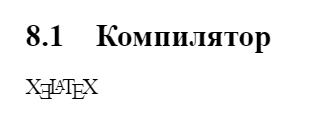
\includegraphics{logo.png}
\caption{Изображение логотипа с разным регистром}
\end{figure}

\item \textcolor{mypink}{graphicx} - для вставки изображения в документ.
\end{itemize}

\section{Собственная команда}

\begin{itemize}
\item $\backslash$mono - команда принимает один аргумент для того, чтобы сделать текст маленьким и моноширинным.
\end{itemize}

\end{document}
